\documentclass[11pt]{article}
\usepackage{graphicx, color}
\usepackage[margin=1in]{geometry}

%Double-spacing
\renewcommand{\baselinestretch}{2.0}


%\textwidth 16.0cm \textheight 9in %23.5cm
%\oddsidemargin 0.1in
%\evensidemargin 0.1in

\newlength{\figratio}
\setlength{\figratio}{1.0in}

\newcommand{\centerfig}[2]{
   \centerline{\resizebox{#2in}{!}{\psfig{file=#1.eps}}}}

\title{Title of Your Paper Goes Here  \\
15-300, Fall 2015
}

\author{Author Name Goes Here}
% To remove the date, uncomment the \date{} command below.
%\date{}


\begin{document}
\maketitle


\section{Introduction}

Describe the context for the three papers.  What is the common problem are
they attempting to solve?  Why is this work important?  

\section{Summary of Paper 1}
\label{ref:paper1-summary}

Here is an example
of how we cite a conference paper by Author1~\emph{et
  al.}~\cite{ConferencePaperExampleTag}.  


\subsection{Approach to solving the problem}
\label{ref:paper1-approach}

\subsection{Summary of results}
\label{ref:paper1-results}

\section{Summary of Paper 2}
\label{ref:paper2-summary}

Here is an example of how we cite
a journal paper by AuthorA~\emph{et al.}~\cite{JournalPaperExampleTag}.

\subsection{Approach to solving the problem}
\label{ref:paper2-approach}

You may want to include illustrations from the papers, if they are helpful,
such as the example shown in Figure~\ref{fig:results-example}.

\begin{figure}[t]
\hrule
\vspace{0.1in}
\centering
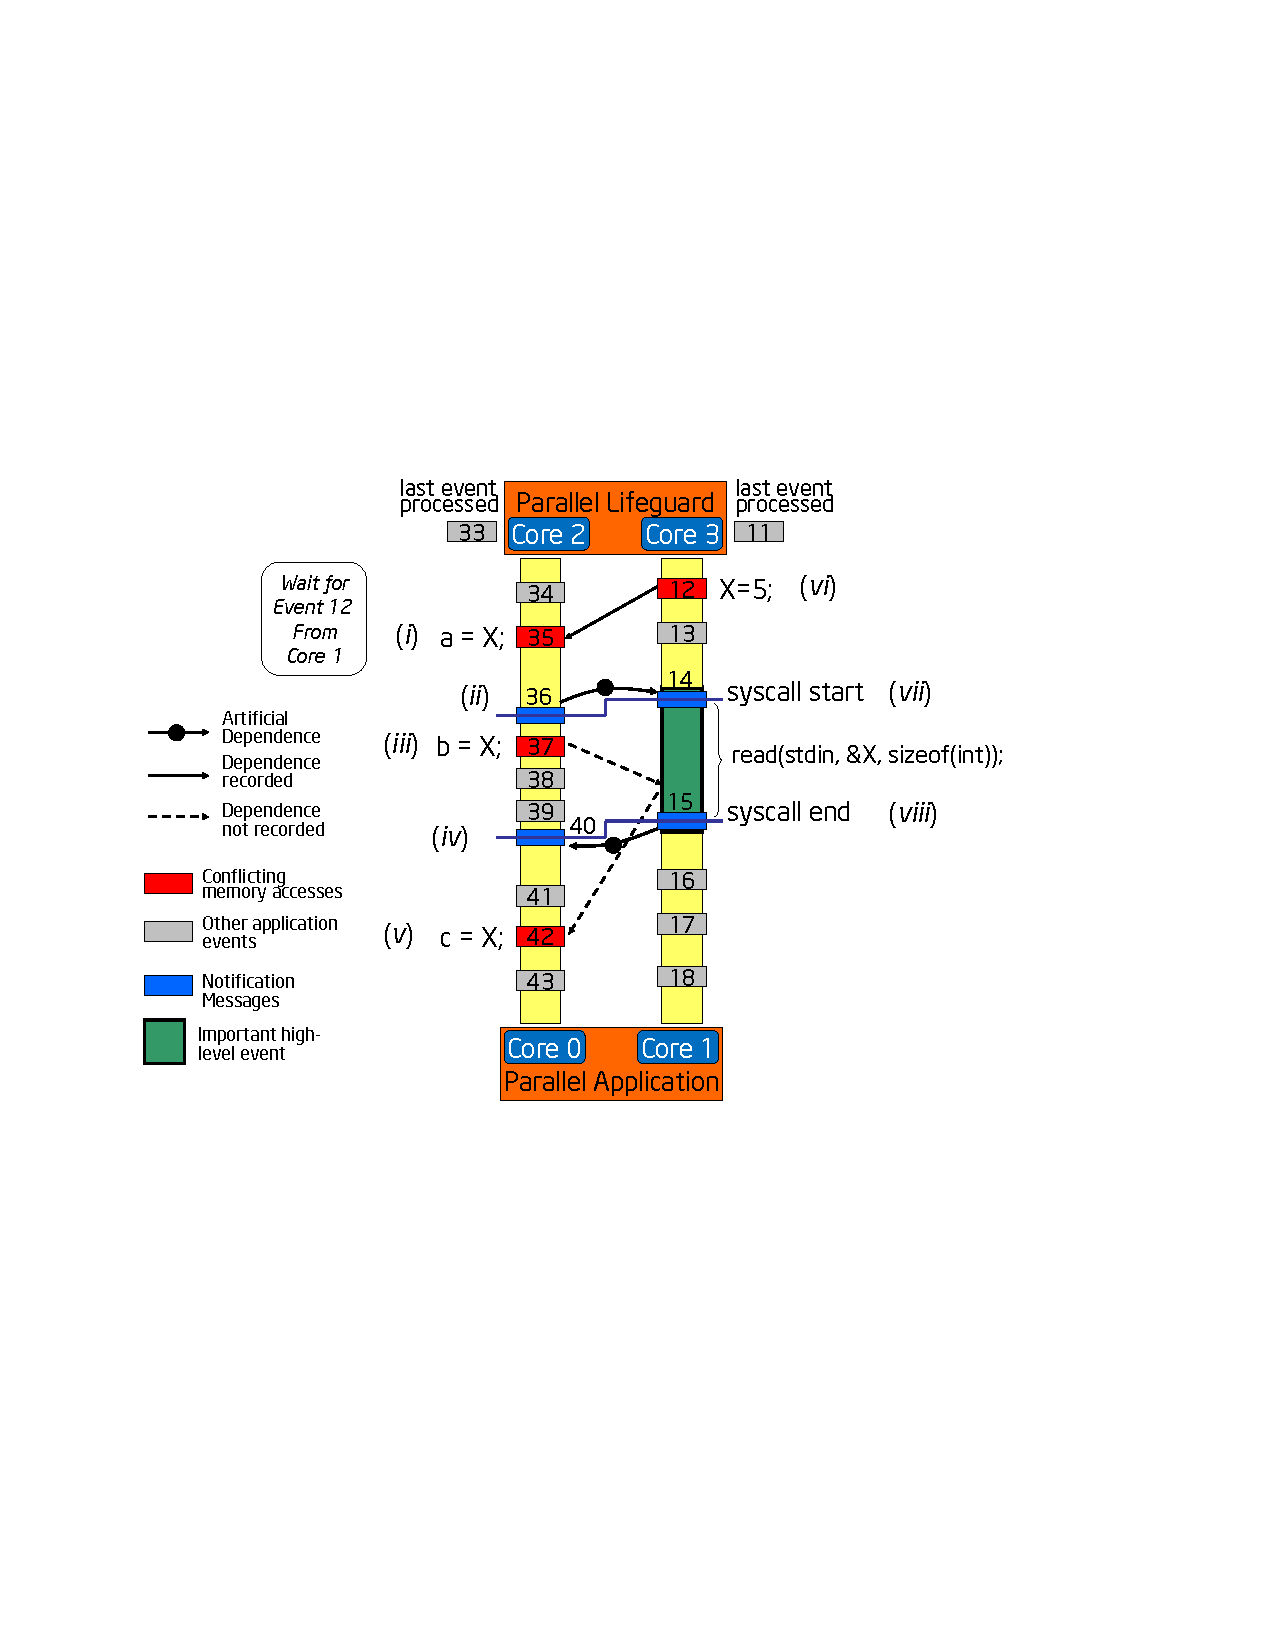
\includegraphics[width=4.0in]{figures/illustration1.pdf}\\
\vspace{0.1in}
\hrule
\caption{Illustration, reproduced from AuthorA~\emph{et al.}~\cite{JournalPaperExampleTag}.}
\label{fig:results-example}
\end{figure}

\subsection{Summary of results}
\label{ref:paper2-results}



\section{Summary of Paper 3}
\label{ref:paper3-summary}

\subsection{Approach to solving the problem}
\label{ref:paper3-approach}

\subsection{Summary of results}
\label{ref:paper3-results}

\section{Comparison of the Three Papers}
\label{ref:comparison-section}

Here you should compare the papers that were discussed earlier in
Sections~\ref{ref:paper1-summary}, \ref{ref:paper2-summary}, and
\ref{ref:paper3-summary}.  You may want to refer back to specific details
in the results sections.  For example, how do the results by
Author1~\emph{et al.}~\cite{ConferencePaperExampleTag} (summarized earlier
in Section~\ref{ref:paper2-results}) compare with the results by
AuthorA~\emph{et al.}~\cite{JournalPaperExampleTag} (summarized above in
Section~\ref{ref:paper1-results}), etc.

\section{Conclusions}
\label{ref:conclusions-section}

What can you conclude from your study?  

\bibliographystyle{plain}
\bibliography{references}

\end{document}

